\newpage
\setcounter{page}{1}
% In this supplementary, we provide details and evaluations of our design choices (Sec. \ref{sec:abl}), along with additional results for BRDF reconstruction with sparse samples (Sec. \ref{sec:add_res}), full reconstruction (Sec. \ref{sec:full_rec}), and compression (See "compression.pdf").

\section{Ablation Studies}\label{sec:abl}
\subsection{Latent Dimension}
We experimented with the dimension size of our latent representations $Z$ on the test dataset for the reconstruction with all available samples and observed that 40-dimensional embeddings give the minimum average mean squared error (See the first row of Table \ref{table: z_abl}). Therefore, we chose our latent space size to be 40. However, we also observed that these can change with the number of sparse samples. For consistency, we kept it same for all our reconstruction results. 

\subsection{Log Relative Mapping (LRM)}\label{sec:lrm}
We apply Log Relative Mapping (LRM) \cite{nielsen2015optimal} to the BRDF data before feeding it the hypernetwork, as described in Section \ref{sec:pre-proc}. We illustrate that LRM improves the reconstruction quality for both PCA and hypernetwork results in Table \ref{table: comparison results} and Figure \ref{fig:qual_comp}. Please note that IPCA is the mapping-applied version of PCA, and "Ours (No LRM)" refers to our results without LRM.


\subsection{Cosine Weighting}
Similar to \cite{ngan2005experimental}, we also weigh the BRDFs with a cosine term based on the assumption of uniform incoming radiance and observed that it offers higher accuracy:

\begin{table}[h]
    \centering
    \caption{Average metric results over the renderings of the test set (20 MERL materials).}

    {\begin{tabular}{l@{\hskip 0.3in}c@{\hskip 0.3in}c@{\hskip 0.3in}c}\toprule
    % \resizebox{0.5\linewidth}{!}{%
    % {\begin{tabular}{ccc}\toprule

 &  No Cosine &  Cosine\\
 \toprule
 PSNR\textuparrow & 33.077 & \cellcolor{blue!25} 33.166 \\
Delta E\textdownarrow & 2.233 & \cellcolor{blue!25} 2.117 \\
SSIM\textuparrow & 0.974 & \cellcolor{blue!25} 0.979 \\
MAE\textdownarrow & 3.908 & \cellcolor{blue!25} 3.492 \\
RMSE\textdownarrow & 7.370 & \cellcolor{blue!25} 6.507 \\
RAE\textdownarrow & 0.098 & \cellcolor{blue!25} 0.089 \\
\bottomrule
    \end{tabular}\par}
    \label{table: cos_abl}
\end{table}

\subsection{Principal Component Analysis (PCA)}
In Section \ref{sec:qual_comp}, we briefly discussed the ablation study we ran to choose the number of principal components for the best-performing IPCA results. Here, we elaborate on the effect of the number of principal components on the performance of IPCA. 


\paragraph{Number of Principal Components:}
We analyzed the optimal number of principal components by initially choosing the same numbers as we did for the ablation study of the latent dimension. Looking at Table \ref{table: z_abl}, we observe that $N_{PC}$ gives the minimum error for sparse cases, where the number of samples $N$ is 40. We further validated
our choice $N_{PC} = 8$ by running IPCA with the number of principal components ranging from 1 to 16 with an incremental change of 1. Figure \ref{fig:ipca_opt} illustrates that $N_{PC} = 8$ still gives the minimum mean squared error (MSE) averaged over the test set.


\begin{figure}[h]
  \centering
  % \fbox{\rule{0pt}{2in} \rule{0.9\linewidth}{0pt}}
   % \includegraphics[width=\linewidth]{fig/different_sample_result_ext.pdf}

  {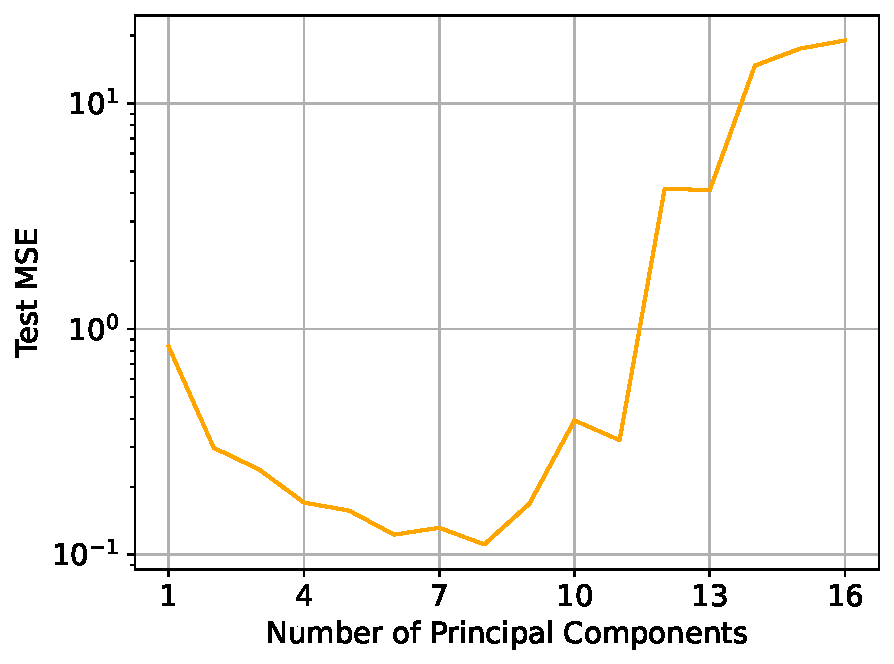
\includegraphics[width=0.5\linewidth]{supp_fig/ipca_opt_q_40_cropped.pdf}}
   \caption{IPCA optimization for the number of principal components.}
   \label{fig:ipca_opt}
\end{figure}

\begin{table*}
    \centering
    \caption{Average Mean squared errors for varying latent space dimensions (first row) and number of principal components (second row)}

    \resizebox{0.9\linewidth}{!}{%
    {\begin{tabular}{l@{\hskip 0.1in}c@{\hskip 0.1in}c@{\hskip 0.1in}c@{\hskip 0.1in}c@{\hskip 0.1in}c@{\hskip 0.1in}c@{\hskip 0.1in}c@{\hskip 0.1in}c}\toprule

 Methods/Dimension & 8 & 20 & 30 & 40 & 50 & 60 & 70 & 80\\
 \toprule
  Ours & 0.073 & \cellcolor{orange!25} 0.046 & 0.062 & \cellcolor{blue!25} 0.045 & 0.051 & 0.053 & 0.049 & \cellcolor{orange!25} 0.046\\
 IPCA & \cellcolor{blue!25} 0.131 & 0.278 & 12.288 & \cellcolor{orange!25} 0.507 & 0.878 & 0.883 & 0.965 & 1.124\\
 % Ours & 0.07316627 & 0.04584484 & 0.062269766 & \cellcolor{blue!25} 0.0450675 & 0.05086073 & 0.05323179 & 0.048830554 & 0.045660965\\
 % IPCA & \cellcolor{blue!25} 0.13114488366971697 & 0.27838688165948045 & 12.287971757668673 & 0.5070392622086964 & 0.8777730931093752 & 0.8827390392824337 & 0.965173480144808 & 1.124261438468366\\
 
% IPCA\textdownarrow & 2.2328 & 2.1167 \\

\bottomrule
    \end{tabular}\par}}
    \label{table: z_abl}
\end{table*}

\subsection{GGX Fittings}
We also fitted an analytic model, GGX \cite{walter2007microfacet}, to the sparse number of measured BRDF samples using a non-linear optimisation (L-BFGS-B method) with Log $l_1$ loss (same loss used in NBRDF). The average PSNR values across our test dataset for varying sample sizes can be found in Table \ref{tab:ggx}. For the results with all samples, we used the dj\_brdf mitsuba plug-in \cite{dupuy2015photorealistic}. Rendering results are also included in this supplementary ("ggx.pdf").


\begin{table}
    \centering
    \caption{GGX - Average metric results over the renderings of our test dataset. We highlight \colorbox{blue!25}{best} results.}

    % \resizebox{0.8\linewidth}{!}
    {%
    {\begin{tabular}{l@{\hskip 0.3in}c@{\hskip 0.1in}c@{\hskip 0.1in}c@{\hskip 0.1in}c@{\hskip 0.1in}c@{\hskip 0.1in}c}\toprule

 % &  NPs &  Ours\\
 % \toprule
 % PSNR & 46.125 & 47.6824 \\
 % Delta E & 2.4238 & 0.5671 \\
 % SSIM & 0.935 & 0.9944 \\

  $N$ &  PSNR \textuparrow & Delta E \textdownarrow & SSIM \textuparrow & MAE \textdownarrow  & RMSE \textdownarrow & RAE \textdownarrow\\ 
 \toprule
 $40$ & 29.198 & 2.821 & 0.924 & 6.724 &  12.778 & 0.141\\
 $160$ &28.893 & 2.831 &  0.923 &6.906 & 13.004 & 0.147\\
 $400$ & 29.193 & 2.771 & 0.924 &  6.722 & 12.798 & 0.141\\
 $2000$ &  29.040 & 2.794 & 0.923 & 6.795 & 12.919 & 0.143\\
 $4000$ & 29.035 & 2.792 & 0.923 & 6.786 & 12.914 & 0.143\\
 All samples & \cellcolor{blue!25} 30.334 & \cellcolor{blue!25}2.241 & \cellcolor{blue!25}0.967 & \cellcolor{blue!25}4.784 & \cellcolor{blue!25}8.787 & \cellcolor{blue!25}0.123\\
\bottomrule
    \end{tabular}\par}}
    \label{tab:ggx}
\end{table}

\section{Additional Results}\label{sec:add_res}

\subsection{Sparse Reconstruction}
In addition to Figure \ref{fig:imp_plots}, we provide MAE, RMSE, and RAE metric plots (Figure \ref{fig:imp_plots_supp}) along with the hypernetwork's average metric results across varying sample sizes (Table \ref{table: ours_diff_samples}). 

\subsection{Full Reconstruction}\label{sec:full_rec}

We first evaluated the full reconstruction capacity of our method by using all available samples during the inference time. Figure \ref{fig:qual_comp} shows our results without/with LRM (Sec. \ref{sec:lrm}) along with the results for Hyper autoencoder (Hyper-AE) \cite{sztrajman2021neural}, PCA, and IPCA. For all methods, we do the same train/test split and compare the methods both qualitatively (Figure \ref{fig:qual_comp}) and quantitatively (Table \ref{table: comparison results}) over the test set. Please note that Hyper-AE is not included in the results for reconstruction with sparse samples since it only works with a fixed grid of input samples, unable to reconstruct materials with varying sizes. 


Figure \ref{fig:qual_comp} shows that our method attains superior results in terms of the reconstruction quality of measured BRDFs. The reconstructed materials with PCA or Hyper-AE cannot capture the material properties, such as the diffuse components, effectively. They can also cause some artifacts (chrome, green-metallic-paint). The linear structure of PCA cannot handle the high dynamic range of the data. Although IPCA \cite{nielsen2015optimal} improves the results substantially, they still have difficulty capturing the right colors. The NBRDF \cite{sztrajman2021neural} reconstruction results can be found in their supplementary. Since our hypernetwork model offers a generalizable approach to NBRDF, it is expected that an overfitting NBRDF model performs better in reconstruction with full samples. 


\begin{table*}
    \centering
    \caption{Hypernetwork - Average metric results across varying sample sizes ($N$) over the test set (Sparse and full reconstruction of unseen materials).}

    \resizebox{0.9\linewidth}{!}{%
    {\begin{tabular}{l@{\hskip 0.2in}c@{\hskip 0.2in}c@{\hskip 0.2in}c@{\hskip 0.2in}c@{\hskip 0.2in}c@{\hskip 0.2in}c}\toprule

 Metrics/$N$ & $8$ & $40$ & $4000$ & $40\,000$ & $640\,000$ & $1\,458\,000$\\
 \toprule
PSNR\textuparrow & 23.090 & 29.822 & 33.170 & 33.019 & \cellcolor{blue!25}33.166 & \cellcolor{orange!25} 33.128 \\
Delta E\textdownarrow & 5.948 & 3.086 & 2.138 & \cellcolor{orange!25} 2.118 & \cellcolor{blue!25}2.117 & 2.181 \\
SSIM\textuparrow & 0.927 & 0.969 & 0.977 & \cellcolor{blue!25} 0.979 & \cellcolor{blue!25} 0.979 & \cellcolor{orange!25}0.978 \\
MAE\textdownarrow & 13.167 & 5.306 & 3.642 & \cellcolor{orange!25} 3.568 & \cellcolor{blue!25}3.492 & 3.574 \\
RMSE\textdownarrow & 22.293 & 9.601 & 6.791 & \cellcolor{orange!25} 6.618 & \cellcolor{blue!25}6.507 & 6.740 \\
RAE\textdownarrow & 0.339 & 0.134 & 0.093 & \cellcolor{orange!25} 0.091 & \cellcolor{blue!25}0.089 & \cellcolor{orange!25} 0.091 \\
\bottomrule
    \end{tabular}\par}}
    \label{table: ours_large_samples}
\end{table*}

\begin{figure*}
  \centering
    {
\includegraphics[width=0.35\linewidth]{fig/legend.png}}\\
  {\includegraphics[width=0.32\linewidth, height=3.cm]{supp_fig/MAE.pdf}}
  {\includegraphics[width=0.32\linewidth, height=3.cm]{supp_fig/RMSE.pdf}}
  \adjustbox{trim={0.\width} {.0\height} {0.\width} {.\height},clip}%
    {\includegraphics[width=0.32\linewidth, height=3.cm]{supp_fig/RAE.pdf}}
   \caption{Average MAE, RMSE, and RAE results across different sample sizes. }
   \label{fig:imp_plots_supp}
\end{figure*}


\begin{table*}
    \centering
    \caption{Quantitative comparison results for full reconstruction over the renderings of the test set.}
        \resizebox{0.9\linewidth}{!}
    {\begin{tabular}{l@{\hskip 0.2in}c@{\hskip 0.2in}c@{\hskip 0.2in}c@{\hskip 0.2in}c@{\hskip 0.2in}c}\toprule
    % {\begin{tabular}{c n{5}{2}n{5}{2}n{5}{2}n{5}{2}n{5}{2}}\toprule
 & Hyper-AE & PCA &  IPCA & Ours (No LRM) & Ours \\
\toprule
 PSNR \textuparrow & 21.696 & 16.407 & 28.471 & 20.696 & \cellcolor{blue!25}33.128 \\
  Delta E \textdownarrow & 7.761 & 13.233 & 4.023 & 8.970 & \cellcolor{blue!25}2.181 \\
 SSIM\textuparrow & 0.873 & 0.818 & 0.975 & 0.896 & \cellcolor{blue!25}0.978 \\
 MAE\textdownarrow & 13.058 & 30.949 & 5.940 & 16.927 & \cellcolor{blue!25}3.574 \\
 RMSE\textdownarrow & 23.051 & 47.018 & 10.276 & 28.314 & \cellcolor{blue!25}6.740 \\
 RAE\textdownarrow & 0.329 & 0.780 & 0.158 & 0.421 & \cellcolor{blue!25}0.091 \\

\bottomrule
    \end{tabular}\par}
    \label{table: comparison results}

\end{table*}
\subsection{Compression}

We report the rendering results of 100 MERL materials for compression (Table \ref{table: oursvsnps}) as a pdf file; see "Compression.pdf".

\subsection{Scene Renderings}
We also rendered multiple scenes \cite{resources16} using our reconstructed materials, including sparse reconstruction, compression and interpolation. The details about the objects covered with our reconstructed materials are as follows (Figure \ref{fig:scene-render}): \textbf{\textit{teapot:}} steel. \textbf{\textit{dragons:}} interpolation of delrin and green-metallic-paint, white marble (dragon paint), silver-metallic-paint3 (ground), dark-red-paint (cloth). \textbf{\textit{cars:}} chrome steel, gold metallic paint3, specular-red-phenolic (car paint), exterior car parts (aluminium), inner wheel (alumina-oxide). \textbf{\textit{kitchen:}} cupboards (natural-209), utensils (chrome), handles, pot, microwave and cooker (two-layer-silver), extractor hood (aluminium), pot and kettle handles (black-obsidian), kettle paint (dark-red-paint), tea towel and cushions (yellow-paint), radio and lamp (polyethylene). \textbf{\textit{living room:}} sofa, coffee table, side tables, wall book shelf (pure-rubber), cushions (green-metallic-paint), twigs (natural-209), legs (dark-specular-fabric).
\textbf{\textit{sofas:}} violet rubber and green latex (sofa cover). 

Renderings can be found in png format under the "scene-renderings" folder.



\begin{figure}[h]
  \centering
  % \fbox{\rule{0pt}{2in} \rule{0.9\linewidth}{0pt}}
   % \includegraphics[width=\linewidth]{fig/different_sample_result_ext.pdf}

  {\includegraphics[width=\linewidth]{supp_fig/SceneRenderings.pdf}}
   \caption{Scene renderings with our reconstructed materials.}
   \label{fig:scene-render}
\end{figure}


% \begin{figure*}[t!]
%     \centering
        
%     \begin{subfigure}[t]{0.8\linewidth}
%     \centering
%     \includegraphics[width=\linewidth]{supp_fig/teapot_scene_v0.png}
%         \caption{Lorem ipsum}
%     \end{subfigure}%
%     \\
%     ~ 
%     \begin{subfigure}[t]{0.5\textwidth}
%         \centering
%         \includegraphics[height=0.7in]{supp_fig/green_sofa_cropped.png}
%         \caption{Sofa cover: green-latex (compression)}
%     \end{subfigure}%
%     ~ 
%     \begin{subfigure}[t]{0.5\textwidth}
%         \centering
%         \includegraphics[height=0.7in]{supp_fig/pink_sofa_cropped.png}
%         \caption{Sofa cover: violet-rubber. Sparse rec. ($N =4000$)}
%     \end{subfigure}
%     \\
%     \begin{subfigure}[t]{\textwidth}
%         \centering
%         \includegraphics[height=2in]{supp_fig/scene_v0_chrome-steel.png}
%         \caption{Lorem ipsum, lorem ipsum,Lorem ipsum, lorem ipsum,Lorem ipsum}
%     \end{subfigure}
%     \\
%     \begin{subfigure}[t]{0.5\textwidth}
%         \centering
%         \includegraphics[height=1.2in]{supp_fig/car_scene_v0_gold.png}
%         \caption{Lorem ipsum}
%     \end{subfigure}%
%     ~ 
%     \begin{subfigure}[t]{0.5\textwidth}
%         \centering
%         \includegraphics[height=1.2in]{supp_fig/car_scene_v0_orange.png}
%         \caption{Lorem ipsum, lorem ipsum,Lorem ipsum, lorem ipsum,Lorem ipsum}
%     \end{subfigure}
    
%     \caption{Scene renderings with our reconstructed materials.}
% \end{figure*}


\begin{figure*}
  \centering
  % \fbox{\rule{0pt}{2in} \rule{0.9\linewidth}{0pt}}
   % \includegraphics[width=\linewidth]{fig/different_sample_result_ext.pdf}
\adjustbox{trim={0.\width} {.\height} {0.\width} {.\height},clip}%
  {\includegraphics[width=0.66\linewidth]{supp_fig/qualitative_comp_40_all_samples.pdf}}
    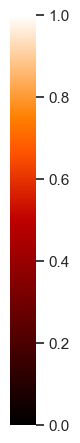
\includegraphics[width=0.02\linewidth]{supp_fig/vbar.png}

   \caption{Qualitative comparison for full reconstruction capacity on the test dataset.}
    % \RM{Why you are not comparing with GGX?}

   \label{fig:qual_comp}
\end{figure*}



% \clearpage
\begin{figure*}
  \centering
  % \fbox{\rule{0pt}{2in} \rule{0.9\linewidth}{0pt}}
   % \includegraphics[width=\linewidth]{fig/different_sample_result_ext.pdf}

  {\includegraphics[width=0.42\linewidth]{supp_fig/supp_40.pdf}}
      % {\includegraphics[width=0.45\linewidth]{supp_fig/supp_40_rms.pdf}}
  {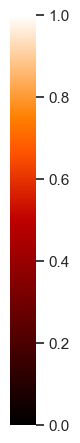
\includegraphics[width=0.02\linewidth]{supp_fig/vbar.png}}
   \caption{Sparse reconstruction results, $N = 40$.}
   \label{fig:40}
\end{figure*}

% \clearpage
\begin{figure*}
  \centering
  % \fbox{\rule{0pt}{2in} \rule{0.9\linewidth}{0pt}}
   % \includegraphics[width=\linewidth]{fig/different_sample_result_ext.pdf}

  {\includegraphics[width=0.42\linewidth]{supp_fig/supp_160.pdf}}
      % {\includegraphics[width=0.45\linewidth]{supp_fig/supp_160_rms.pdf}}
  {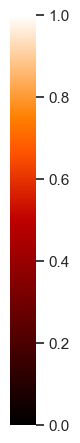
\includegraphics[width=0.02\linewidth]{supp_fig/vbar.png}}
   \caption{Sparse reconstruction results, $N = 160$.}
   \label{fig:160}
\end{figure*}

% \clearpage
\begin{figure*}
  \centering
  % \fbox{\rule{0pt}{2in} \rule{0.9\linewidth}{0pt}}
   % \includegraphics[width=\linewidth]{fig/different_sample_result_ext.pdf}

  {\includegraphics[width=0.42\linewidth]{supp_fig/supp_400.pdf}}
      % {\includegraphics[width=0.45\linewidth]{supp_fig/supp_400_rms.pdf}}
  {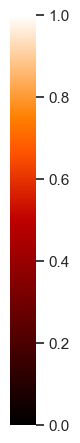
\includegraphics[width=0.02\linewidth]{supp_fig/vbar.png}}
   \caption{Sparse reconstruction results, $N = 400$.}
   \label{fig:400}
\end{figure*}

% \clearpage
\begin{figure*}
  \centering
  % \fbox{\rule{0pt}{2in} \rule{0.9\linewidth}{0pt}}
   % \includegraphics[width=\linewidth]{fig/different_sample_result_ext.pdf}

  {\includegraphics[width=0.42\linewidth]{supp_fig/supp_2000.pdf}}
      % {\includegraphics[width=0.45\linewidth]{supp_fig/supp_2000_rms.pdf}}
  {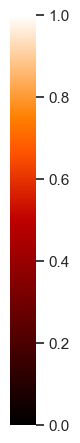
\includegraphics[width=0.02\linewidth]{supp_fig/vbar.png}}
   \caption{Sparse reconstruction results, $N = 2000$.}
   \label{fig:2000}
\end{figure*}

\begin{figure*}
  \centering
  % \fbox{\rule{0pt}{2in} \rule{0.9\linewidth}{0pt}}
   % \includegraphics[width=\linewidth]{fig/different_sample_result_ext.pdf}

  {\includegraphics[width=0.42\linewidth]{supp_fig/supp_4000.pdf}}
    % {\includegraphics[width=0.45\linewidth]{supp_fig/supp_4000_rms.pdf}}
  {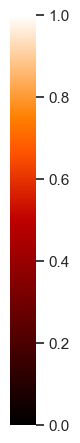
\includegraphics[width=0.02\linewidth]{supp_fig/vbar.png}}
   \caption{Sparse reconstruction results, $N = 4000$.}
   \label{fig:4000}
\end{figure*}


